% Diese Zeile bitte -nicht- aendern.
\documentclass[course=erap]{aspdoc}

%%%%%%%%%%%%%%%%%%%%%%%%%%%%%%%%%
%% TODO: Ersetzen Sie in den folgenden Zeilen die entsprechenden -Texte-
%% mit den richtigen Werten.
\newcommand{\theGroup}{IhreGruppennummer} % Beispiel: 42
\newcommand{\theNumber}{IhreProjektnummer} % Beispiel: A123
\author{Vorname1 Nachname1 \and Vorname2 Nachname2 \and Vorname3 Nachname3}
\date{AktuellesSemester} % Beispiel: Wintersemester 2019/20
%%%%%%%%%%%%%%%%%%%%%%%%%%%%%%%%%

% Diese Zeile bitte -nicht- aendern.
\title{Gruppe \theGroup{} -- Abgabe zu Aufgabe \theNumber}

\usepackage{graphicx} 
\usepackage{subcaption}
\graphicspath{{images/}}

\begin{document}
\maketitle

\section{Einleitung}
Der Schwerpunkt dieses Projekts liegt auf der Konvertierung farbiger Bilder in Graustufen und der darauf folgenden Durchführung einer Tonwertkorrektur. 
Als Eingabe lesen wir zuerst 24bpp PPM (P6) Pixelbilder. Jeder Farbpixel wird als Vektor mit den drei Farbkanälen Rot R, Grün G und Blau B definiert. Durch die Berechnung eines gewichteten Durchschnitts D, wandeln wir zunächst die Bilder in Graustufen um. Die entstandenen Graustufenbilder unterziehen wir dem Tonwertkorrektur mittels eine Interpolationsfunktion, die ermöglicht eine reibungslose Anpassung der Graustufenwerte zwischen den nutzerspezifizierte Stützpunkten. 
Zuletzt erstellen wir eine neue Datei im 8bpp PGM (P5) Format und dort hineinschreiben wir die berechneten Werte nach dem Tonwertkorrektur.

\begin{figure}[h]
    \begin{subfigure}{0.5\linewidth}
      \centering
      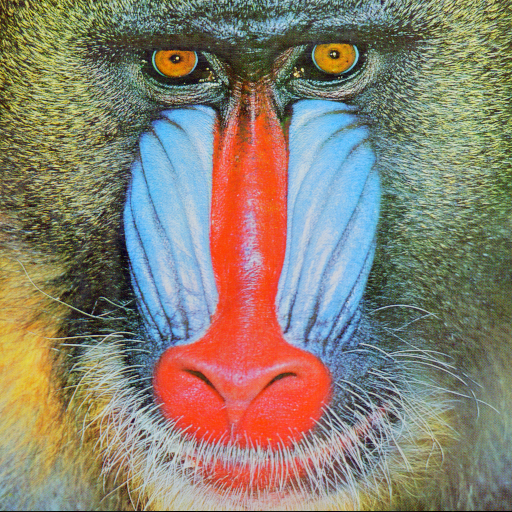
\includegraphics[width=\linewidth]{mandrill-2}
      \caption{EingabeBild}
      \label{fig:eingabe}
    \end{subfigure}%
    \begin{subfigure}{0.5\linewidth}
      \centering
      \includegraphics[width=\linewidth]{mandrillausgabe}
      \caption{AusgabeBild}
      \label{fig:ausgabe}
    \end{subfigure}
\end{figure}

Die Abbildungen \ref{fig:eingabe} und \ref{fig:ausgabe} repräsentieren ein Eingabebild und das entsprechende Ergebnis unserer Hauptimplementierung unter Verwendung der Standardwerte für Schwarz-, Weiß- und Mittelwerte für die Tonwertkorrektur.

In den kommenden Abschnitten werden wir die gewählten Ansätze erläutern, die korrektheit und die Genauigkeit der Hauptimplementierung prüfen und das Laufzeitverhalten und die Performanz evaluieren.


\section{Lösungsansatz}
\subsection{Graustufen Konvertierung}

\subsubsection{Intuitiver Ansatz: Durchschnitt}
die folgende Umrechnungsformel ist einfach der Durchschnitt der RGB Komponenten:
 \[ D = (R + G + B) / 3  \]
Die Durchschnittsmethode ist ebenfalls problematisch, da sie jedem Komponenten den gleichen Gewicht zuweist.

\subsubsection{Grün-Kanal Ansatz}
Das menschliche Auge ist am empfindlichsten gegen Grün, daher ist die Verwendung von Grün eine schnellere , aber ungenauere  Alternative zur Umwandlung von RGB in Luminanz.
\[D = G\] 

\subsubsection{Luminanz Ansatz}
Die Luminanz $Y$ dient als Maß für die Helligkeit von Bildpunkten, entsprechend der Wahrnehmung durch das menschliche Auge. Da das Auge besonders empfindlich für die Farbe Grün ist und weniger empfindlich für Blau, wird eine Gewichtung der RGB-Komponenten benötigt, um die Farbwahrnehmung des menschlichen Auges zu berücksichtigen. [1]
In unserem Kontext, bei der Arbeit mit einem PPM-Bild, das der ITU-R-Empfehlung BT.709 entspricht [2], wird die folgende Umrechnungsformel gemäß Rec. 709 für die Berechnung der CIE-Luminanz aus den linearen RGB-Komponenten verwendet:
 \[Y = 0.2125R + 0.7154G + 0.0721B \] [3]
Die ITU-R Empfehlung BT.709 definiert auch das gamma-codierte Luma $Y'$, die eine gewichtete Summe der nichtlinearen (nach Gamma-Korrektur) RGB-Komponenten entspricht, wobei gilt:
 \[Y' = 0.2126R' + 0.7152G' + 0.0722B' \] [4]
Die Verwendung der Luminanz bietet eine genauere Darstellung der tatsächlichen Helligkeit und eignet sich daher besser für die 8-Bit-Kodierung von Graustufen. Man muss jedoch das Bild zuvor in einen linearen RGB-Farbraum umwandeln, um den gewichteten Durchschnitt auf die linearen RGB-Komponenten anwenden zu können.
Alternativ kann jede der drei Farbkomponenten auf das berechnete Luma Y' gesetzt werden. Dies ermöglicht eine einfachere Berechnung und ist in der Praxis oft ausreichend für Graustufenbilder.
 \[ D = Y' = 0.2126R' + 0.7152G' + 0.0722B' \]    \[0.2126 + 0.7152 + 0.0722 = 1\]




% TODO: Je nach Aufgabenstellung einen der Begriffe wählen
\section{Korrektheit/Genauigkeit}


\section{Performanzanalyse}


\section{Zusammenfassung und Ausblick}

% TODO: Fuegen Sie Ihre Quellen der Datei Ausarbeitung.bib hinzu
% Referenzieren Sie diese dann mit \cite{}.
% Beispiel: CR2 ist ein Register der x86-Architektur~\cite{intel2017man}.
\bibliographystyle{plain}
\bibliography{Ausarbeitung}{}

\end{document}
